\chapter{The no-arbitrage band: costs, capital and position limits}\label{ch:band}
\chapterlead{The band within which the basis moves in normal times, and how it relates to the three slow-moving limits:
trading costs, arbitrage capital and the position-limit regime. The chapter uses non-ban stock-days only, except where it
counts bans.}

\section{Estimating the band}
Let $x_{t-1}$ be yesterday's basis minus the stock's median basis on non-ban days, in basis points, and $\Delta m_t$ the
change in the basis of the same contract. The three-regime threshold model is
\[ \Delta m_t=a_r+\rho_r x_{t-1}+e_t,\qquad r=\begin{cases}\text{lower} & x_{t-1}<g_L\\ \text{middle} & g_L\le x_{t-1}\le g_U\\ \text{upper} & x_{t-1}>g_U,\end{cases} \]
with the thresholds chosen to minimise the sum of squared residuals over a grid of percentiles of $x$ (at least 10\% of
observations in each outer regime and 20\% in the middle). Linearity is tested with a sup-$F$ statistic whose distribution
under the linear model comes from a wild bootstrap clustered by date; threshold intervals come from resampling whole
stocks. I also estimate exponential and logistic smooth-transition models (Tse, 2001), in which the speed of reversion
changes smoothly with the deviation, and models in which it changes smoothly with an observed state.

\begin{table}[t]
\caption[Pooled threshold model of the basis]{The basis moves in a wide, asymmetric band, but much of the daily reversion is noise}\label{tab:setar}
\exsub{Pooled three-regime threshold model, non-ban days, 2015 to 2026 (473,110 observations, 360 stocks)}
\small\begin{tabular}{@{}>{\raggedright\arraybackslash\bfseries\color{accent}}p{6.4cm}ccc@{}}
\toprule
& \thd{Lower regime} & \thd{Middle regime} & \thd{Upper regime} \\
\midrule
Threshold (bp, relative to the stock's median) & below $-34.5$ & & above $+23.9$ \\
95\% interval (stock bootstrap) & $[-37.2,\,-32.2]$ & & $[+20.3,\,+26.1]$ \\
Share of observations & 0.12 & 0.76 & 0.12 \\
Slope of $\Delta m_t$ on $x_{t-1}$ & $-0.084$ & $-0.468$ & $-0.809$ \\
Slope, instrumented by $x_{t-2}$ & $-0.121$ & $-0.192$ & $-0.141$ \\
\bottomrule
\end{tabular}
\exsource{Thresholds chosen by least squares over a grid of percentiles; intervals from resampling whole stocks. Source: author's calculations.}
\end{table}

\begin{figure}[t]
\caption[Daily change in the basis against its deviation]{The further the basis moves from the stock's median, the more it reverts the next day}\label{fig:bandscatter}
\exsub{Mean change in the basis today by yesterday's deviation from the stock's median (5\bp\ bins), non-ban days; shaded: the estimated band}
\centering\includegraphics[width=\linewidth]{fig_band_scatter}
\exsource{Source: author's calculations.}
\end{figure}

Linearity is rejected (sup-$F$ 7,471 against a bootstrap 95\% critical value of 31). The band is about 58\bp\ wide and
asymmetric: the lower edge is further from the centre, as expected when reverse arbitrage is costlier than cash-and-carry.
By the Bayesian information criterion the threshold model fits best, the logistic smooth-transition model (slow reversion
below $+5$\bp, fast above) almost as well, and the symmetric exponential model clearly worse; a symmetric smooth transition
does not suit an asymmetric band.

The slopes need care. Inside the band the model of Chapter~\ref{ch:theory} predicts almost no correction, yet the middle
slope implies a half-life of about one day. Daily volume-weighted prices contain noise, and classical noise biases these
slopes toward $-1$. Instrumenting $x_{t-1}$ with $x_{t-2}$ (last row of Table~\ref{tab:setar}, with regimes classified by
$x_{t-2}$) shrinks all three slopes and removes most of the difference between the upper and lower regimes. Much of the
day-to-day reversion is therefore noise, and the slower reversion of cheap futures in the threshold model is not a robust
finding. The thresholds, which describe where the basis spends its time, are less affected.

\begin{figure}[t]
\caption[Estimated band edges by year]{The band is stable from year to year, apart from the dislocation of March 2020}\label{fig:bandyears}
\exsub{Thresholds of the pooled threshold model by calendar year, non-ban days, basis relative to each stock's median}
\centering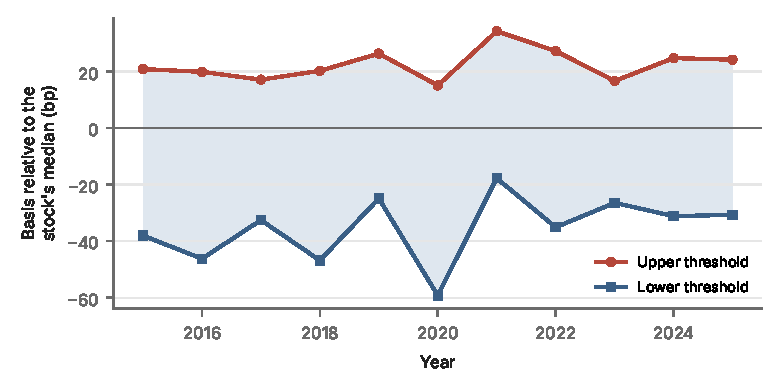
\includegraphics[width=\linewidth]{fig_band_years}
\exsource{Source: author's calculations.}
\end{figure}

The band is stable across years (Figure~\ref{fig:bandyears}), apart from 2020, when the March dislocation pushed the lower
edge to $-59$\bp. The lower edge is wider far from expiry ($-40$\bp\ with 17 or more trading days left against $-28$\bp\
in the last ten days), in line with edges that shrink as expiry approaches. In a smooth-transition model with the number
of trading days to expiry as the state, reversion is faster in the last week (the slope rises by 0.22 above seven days,
s.e.\ 0.02).

\section{Costs}
\paragraph{Pre-specified test (H3).} Around each STT increase I compare each stock's 80th percentile of the basis in the 40
trading days before and the 40 from the event.
\begin{table}[t]
\caption[Change in stock-level percentiles of the basis around STT increases]{The upper part of the basis rose after the 2024 and 2026 tax increases}\label{tab:h3}
\exsub{Mean change in each stock's percentiles of the basis, 40 trading days after against 40 before (bp)}
\small\begin{tabular}{@{}>{\bfseries\color{accent}}lccccc@{}}
\toprule
\thd{Event} & \thd{STT change} & \thd{Stocks} & \thd{80th percentile} & \thd{20th} & \thd{Median} \\
\midrule
3 Apr 2023$^{a}$ & $+0.25$ & 181 & $-2.12$ & $+0.24$ & $+0.27$ \\
1 Oct 2024 & $+0.75$ & 172 & $+6.42$ & $+4.55$ & $+5.39$ \\
1 Apr 2026 & $+3.0$ & 192 & $+7.44$ & $+2.10$ & $+6.30$ \\
\bottomrule
\end{tabular}

\exsource{$^{a}$ Same day as the change in the taxation of debt funds; reported, not used as evidence. STT change in bp of the futures sale. Source: author's calculations.}
\end{table}
Pooling 2024 and 2026, the mean change in the 80th percentile is $+6.96$\bp\ (s.e.\ 0.61, clustered by stock), and the
ordering of the three events matches the size of the cost changes. On the pre-specified statistic H3 is supported. The
pre-specified placebo, the same statistic at 30 dates away from the true events, tells a more cautious story: shocks common
to all stocks move the whole distribution, the placebo statistic has a standard deviation of 7.4\bp, and the true changes
rank at the 10th and 7th percentiles of the placebo distribution (Figure~\ref{fig:h3placebo}). The changes in the band's width and in the upper
percentile relative to the median are not unusual. The rise is mostly a shift of the whole distribution, larger than the
cost changes, and standard errors clustered only by stock overstate the precision when every observation shares the same
event date (Kolari and Pynn\"onen, 2010).

\begin{figure}[t]
\caption[The STT events against placebo dates]{Against placebo dates, the rise after the tax increases is large but not exceptional}\label{fig:h3placebo}
\exsub{Mean change in stocks' 80th percentile of the basis at the three STT dates and at 30 placebo dates (bp)}
\centering\includegraphics[width=\linewidth]{fig_h3_placebo}
\exsource{Placebo dates every 80 trading days, away from the true events. Source: author's calculations.}
\end{figure} As a further check, the same statistic at the three dates of SEBI's 2024 to 2025
reforms of index derivatives, which did not change the costs of single-stock arbitrage, gives $-4.1$, $-0.3$ and
$+1.9$\bp, all well inside the placebo range.

\paragraph{Band edges by tax period.} Measuring each deviation from the stock's median within each period (the full-sample
median does not remove the 2026 level shift), the upper threshold is $+23.8$, $+18.9$, $+23.1$ and $+28.9$\bp\ in the four
STT periods and the lower threshold $-39.1$, $-30.9$, $-31.5$ and $-31.5$\bp. The upper edge is highest in the
highest-tax period but does not rise step by step with the tax. Reversion above the upper edge weakens over time (slope
$-0.77$, $-0.55$, $-0.20$, $-0.15$), which coincides with both rising costs and rising arbitrage capital.

\paragraph{A bottom-up cost band.} The full round trip of an overnight cash-and-carry position (STT of 0.1\% on the cash
purchase and on delivery at expiry, STT on the futures sale, stamp duty, exchange charges, the SEBI fee, GST and an
institutional brokerage of 0.01\% per leg) costs 27.1, 27.3, 28.0 and 31.0\bp\ in the four periods (25 to 38\bp\ for
brokerage between 0.005\% and 0.03\% per leg). Rolling an existing position for one more month costs 4.0 to 8.0\bp. The
estimated upper threshold in levels ($+22$ to $+28$\bp) and the 80th percentile lie below the full round trip, which sits
between the 90th and 95th percentiles. New capital enters only at large deviations; funds that keep capital in place and
roll can lean against much smaller ones. This is one reason why fixed thresholds sit inside the full cost band, as the
model's inventory result implies (Figure~\ref{fig:costband}).

\begin{figure}[t]
\caption[The bottom-up cost of a cash-and-carry position]{The full cost of a new position lies above the estimated upper edge}\label{fig:costband}
\exsub{Round trip of an overnight cash-and-carry position held to delivery, by STT period (bp of notional); triangles: estimated upper threshold in levels}
\centering\includegraphics[width=\linewidth]{fig_cost_band}
\exsource{Institutional brokerage of 0.01\% per leg; GST of 18\% on fees and brokerage. Source: NSE circulars on STT and transaction charges; author's calculations.}
\end{figure}

\section{Arbitrage capital}
\paragraph{Pre-specified test (H4).} Monthly, from May 2018 to September 2026, I regress the 80th percentile of the basis
across all non-ban stock-days on last month's net inflow into arbitrage funds as a share of their assets, with step
dummies for April 2023, October 2024 and April 2026. The coefficient is $-17.5$\bp\ per unit of flow (Newey-West s.e.\ 14.2,
one-sided $p=0.11$): a 10\% inflow goes with a 1.7\bp\ lower upper quantile the next month. In first differences the
relation is clearer ($-20.6$, s.e.\ 6.8), and it is visible before April 2023 ($-26.0$, s.e.\ 16.5) but not after
($+17.1$, s.e.\ 16.9). Same-month flows have a positive coefficient, as expected when flows chase the returns that a rich
basis offers. With about a hundred months the test has little power (Figure~\ref{fig:h4}).

\begin{figure}[t]
\caption[Arbitrage-fund flows and the upper tail of the basis]{The upper tail of the basis and arbitrage-fund flows move a great deal from month to month}\label{fig:h4}
\exsub{Monthly 80th percentile of the basis across non-ban stock-days (top) and net inflow into arbitrage funds as a share of assets (bottom); dashed: April 2023}
\centering\includegraphics[width=\linewidth]{fig_h4_flows}
\exsource{Source: AMFI monthly reports; NSE bhavcopies; author's calculations.}
\end{figure}

\paragraph{Capital as a state.} In a smooth-transition model with log arbitrage-fund assets as the state, reversion is
faster when assets are large (the slope falls by 0.077, s.e.\ 0.019, above about Rs 95,000 crore). This variable also orders
time, so the evidence is descriptive.

\paragraph{Peak margins.} From December 2020 to September 2021 margins had to be collected on peak intraday positions, in
four steps of 25\%. This raises the capital an arbitrageur must post during the day. The upper percentile moves in both
directions at the four steps ($+3.3$, $+9.6$, $-9.9$ and $+3.5$\bp, against a placebo standard deviation of 7.4), so I find
no consistent effect; the rule mainly binds intraday leverage, which a daily basis does not measure.

\section{Position limits}
\paragraph{Anticipation (H9).} On non-ban days before October 2025, the share of days on which a stock's basis is in its own
upper tail (above the 80th percentile of its days with utilisation below 60\%) rises from 0.20 to about 0.27 as utilisation
the day before approaches 95\% (Figure~\ref{fig:h9}). With stock and date fixed effects, the slope of this share on
utilisation between 0.60 and 0.95 is $+0.079$ (s.e.\ 0.038, one-sided $p=0.019$), the lower tail does not change, and the
increase comes more as a step around 0.75 than as a smooth slope. The basis is more often rich as the trigger nears, as
the anticipation result predicts, although high utilisation also signals demand pressure. In a smooth-transition model
with utilisation as the state, reversion weakens as utilisation rises (the slope rises by 0.225, s.e.\ 0.053).

\begin{figure}[t]
\caption[The basis as utilisation nears the trigger]{Rich futures become more common as utilisation approaches the 95\% trigger}\label{fig:h9}
\exsub{Share of non-ban days with the basis in the stock's upper and lower tail, by utilisation the day before (raw shares, before October 2025)}
\centering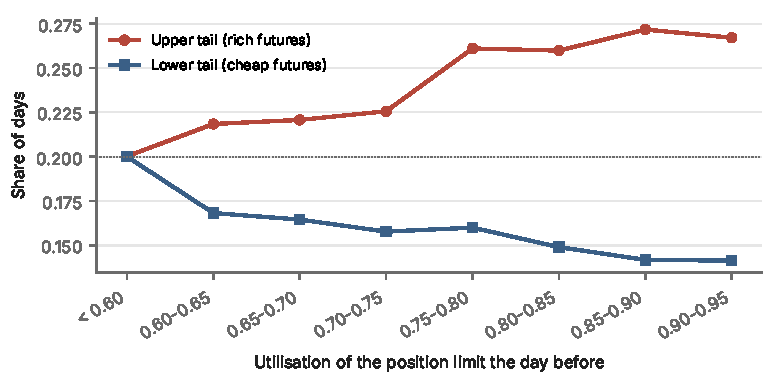
\includegraphics[width=\linewidth]{fig_h9_tails}
\exsource{With date fixed effects the lower-tail decline disappears; the upper-tail rise remains. Source: author's calculations.}
\end{figure}

\paragraph{The October 2025 formula and quarterly resets.} The size of each stock's MWPL cut on 1 October 2025 (0.24 to
0.69 log points) raised its utilisation strongly (first stage $+0.28$ per unit, s.e.\ 0.03). Its effect on the upper tail is
$+0.061$ (s.e.\ 0.050, $p=0.11$), on the level $+4.8$\bp\ and on bans $+0.023$: all in the predicted direction, none
significant. The quarterly resets of January, April and July 2026 move utilisation but show no effect on the basis.

\paragraph{How the October 2025 rules changed the number of bans.} SEBI's stated aim was to reduce ``spurious'' bans. Before
the reform, bans were driven by open interest, not by changes in the limit: on the day utilisation crossed 95\% the limit
fell for only 8 of 1,744 entries, and only 7 (0.4\%) would not have crossed at the previous day's limit. To see what the
two parts of the reform did, I simulate the ban rule (enter the day after utilisation exceeds 95\%, leave the day after it
is at or below 80\%) for the stocks that were in the segment on both 30 September and 1 October 2025. Applied to the actual
utilisation, the simulation reproduces the official ban lists exactly. I then apply it with open interest measured gross
or in delta terms, and with the new limit or the limit the old formula would have given (each stock's new limit scaled by
its ratio of old to new limit on 1 October 2025, an approximation).

\begin{table}[t]
\caption[Bans under the new rule and under counterfactual rules]{The new rule produced about a quarter of the ban days the old rule would have}\label{tab:spurious}
\exsub{Bans from 1 October 2025 to 27 October 2026 for the stocks in the segment on 30 September and 1 October 2025}
\small\begin{tabular}{@{}>{\bfseries\color{accent}}lccc@{}}
\toprule
\thd{Open interest and limit} & \thd{Ban stock-days} & \thd{Spells} & \thd{Stocks} \\
\midrule
Delta-adjusted, new limit (the actual rule) & 412 & 45 & 11 \\
Gross, old-formula limit (the old rule) & 1,505 & 112 & 36 \\
Gross, new limit & 6,256 & 296 & 85 \\
Delta-adjusted, old-formula limit & 1 & 1 & 1 \\
\bottomrule
\end{tabular}

\exsource{The 45 spells include one that began on 30 September 2025. Simulated ban rule validated against the official lists. Source: NSE combined open interest files; author's calculations.}
\end{table}

\begin{figure}[t]
\caption[Ban days under four rules]{Measuring open interest in delta terms removes almost all bans; the lower limit alone would have multiplied them}\label{fig:spurious}
\exsub{Ban stock-days, 1 October 2025 to 27 October 2026, under the actual and three counterfactual rules}
\centering\includegraphics[width=\linewidth]{fig_spurious}
\exsource{Source: as for Table~\ref{tab:spurious}.}
\end{figure}

Under the old rule the same stocks would have spent about 3.7 times as many days in a ban (Table~\ref{tab:spurious}).
The two parts of the reform pull in opposite directions: measuring open interest in delta terms removes almost every
ban, because options now count only by their delta and offsetting positions of the same client net out, while the lower limit on its own would have quadrupled them.
The combination cut bans by about three quarters.

\paragraph{The 2020 halving and restoration.} From 23 March 2020 the limit was halved for stocks whose recent daily
price range or utilisation was high, and on 27 November 2020 it was restored for the 70 stocks whose limit was then
halved. The restoration is a clean shock: it was
announced, it came in a calm market, and it doubled the limit of some stocks and not others. Against other F\&O stocks, in
the 40 trading days either side, the utilisation of the restored stocks fell by 0.21 (s.e.\ 0.02), their share of days in
a ban by 4.6 percentage points (s.e.\ 1.4), and the share of days with their basis in its upper tail by 6.8 percentage
points (s.e.\ 3.2). The basis level did not change significantly ($-2.8$\bp, s.e.\ 3.1). A false restoration date 20 days
earlier shows no effect on utilisation, bans or the upper tail. A looser limit makes rich futures less common, as the
anticipation result predicts, although the upper-tail effect is weaker with a 20-day window ($-6.1$, s.e.\ 4.0). The
halving itself coincided with the March 2020 crash and selected stocks on the outcomes, so I do not interpret it.

\begin{figure}[t]
\caption[The 2020 restoration of the position limit]{Restoring the limit cut the utilisation of the affected stocks at once}\label{fig:covid}
\exsub{Mean utilisation of the MWPL for the 70 stocks whose limit was restored on 27 November 2020 and for other F\&O stocks}
\centering\includegraphics[width=\linewidth]{fig_covid}
\exsource{The fall on day 0 is mechanical (the denominator doubled); the tests use bans and the basis. Source: NSE combined open interest files; author's calculations.}
\end{figure}

\section{Frictions across stocks (H1)}
For F\&O stocks I build a quarterly friction index from the spread, illiquidity, idiosyncratic volatility, utilisation of
the position limit and SLB scarcity, measured in the previous quarter. A one standard deviation higher index goes with a
band (80th minus 20th percentile of the basis) 3.5\bp\ wider (s.e.\ 1.1, one-sided $p=0.002$; mean 40.8\bp) and a mean
absolute basis 2.5\bp\ larger. The relation is across stocks: with stock fixed effects it disappears. The persistence
measure moves the wrong way, which the noise result above explains, and SLB scarcity enters with the wrong sign, which
suggests that SLB activity reflects demand to borrow. Per-stock threshold models (258 stocks) give a median band of $-26$ to
$+17$\bp, and their widths are not related to the stocks' average index.

\section{Summary}
The basis follows a wide, asymmetric, nonlinear band. Its edges respond to costs less cleanly than the model implies; the
full cost of new arbitrage lies in the outer tail, while the cost of keeping capital in place is small. Capital and the
position-limit regime leave traces in the predicted direction (faster correction with more capital, a richer basis near
the trigger, a less often rich basis after the 2020 restoration of the limit), but the formal tests of capital flows and of
the 2025 reform are not significant. The 2025 rules cut the number of bans by about three quarters.
